\documentclass[pageno]{jpaper}

%replace XXX with the submission number you are given from the ISCA submission site.
%\newcommand{\iscasubmissionnumber}{333}

\usepackage[normalem]{ulem}


\begin{document}

\title{CG-Sharing: Efficient Content Sharing in GPU-Based Cloud Gaming}

\date{}
\maketitle

%\thispagestyle{empty}

\begin{abstract}
With the fast development of the GPU server technology, cloud gaming has come to the era and become popular in recent years. Unlike the traditional desktop gaming where the graphic rendering is performed locally using the user's personal graphics card, cloud gaming environment tends to run distributed games to support many users at the same time in the cloud gaming center where most of the rendering jobs are done in the remote GPU cluster. The rendered frames are streamed to user's devices such as notebooks, tablets and cell phones. For the economic cloud gaming to be viable, the operator must make full utilization of the expensive hardware resources like the graphic cards, and the state of art technology tries to render multiple instances of games on the same GPU. In this paper, we first identify that there are many redundant and duplicated contexts/workloads existing in today's cloud gaming rendering that waste a large amount of memory bandwidth and system energy. We in turn propose novel system and architecture enhancements to effectively share the contents across the game instances from different users in the cloud gaming center. Our experiment shows 31.84\% decrease in the DMA transfers, 26.89\% reduction of video memory usage, 8.99\% increase in the gaming performance and 8.51\% cutdown of the system power consumption in the GPU server using our proposed content sharing methodology.
\end{abstract}

\section{Introduction}

Cloud gaming \cite{wiki}, also known as Gaming on Demand or Gaming as a Service, is an online gaming style that allows on-demand streaming of games onto target devices such as notebooks, tablets and cell phones. This is similar to Video on Demand. The control events from mice, keyboards, joysticks and touch-screens are transmitted from the devices back to the cloud gaming servers. Unlike the traditional gaming experience where the graphic rendering is performed locally using the player's own graphic card, the actual scenes in cloud gaming are rendered in the GPU servers and are streamed directly to the client. The most commonly used technology for cloud gaming are video streaming and file streaming. For most of the popular cloud gaming platforms \cite{OnLive}\cite{Gaikai}, video streaming is chosen because it is less demanding in terms of the device capability and bandwidth.

It is a rather new concept that recently gains popularity with consumers due to the ever-improving availability of sufficient networking infrastructure to meet the high requirements for bandwidth and latency. This service takes the advantage of the broadband connection, powerful server clusters and the video stream compression to stream the high-quality game contents to a subscriber's device. Users can play without acquiring the actual game because the game code is executed primarily in the server cluster. As a result, the subscriber can use a less powerful device to play a fancy 3D game which is normally not possible to run locally, since the server does all the heavy-lifting workloads for subscriber's device. Most cloud gaming platforms are private and proprietary such as OnLive and Gaikai \cite{OnLive}\cite{Gaikai}. The first open source cloud gaming platform was not released until April, 2013 \cite{GamingAnywhere}. The forecasted cloud gaming market value can be as high as 24.75 Billion USD \cite{marketShare}.


On the other hand, GPU vendors such as NVIDIA have begun to provide cloud gaming data centers with custom hardware targeting at a greater efficiency for concurrent games per grid node. With NVIDIA Grid technology \cite{nvgrid}, the first product that supports cloud-gaming, the GPU utilization ratio is about two simultaneous users per graphics card. For each server rack, it can hold 480 users and consume between 800 and 900 watts power per blade \cite{gridNews}. Obviously, this kind of low hardware utilization ratio and power-hungry cloud gaming service is not financially competitive enough for ordinary users to switch from conventional gaming style to the more advanced cloud gaming \cite{radeonsky}\cite{gridNews}.


 One major reason behind that is today's cloud gaming products are architecturally based on commercial graphics cards which are designed for one application at a time. These products fail to recognize the fact of the concurrency between different users who play the same game in the cloud gaming environment. Due to the nature of the ``single player/single device'' model prior to the advent of cloud gaming, a system was rarely required to execute multiple instances of a single game concurrently. Existing resource management solutions from the hardware architecture to the system driver mostly consider the optimal usage of GPU resources for a single application, but fail to take into account that applications from multiple users might operate on a big set of overlapping data. For example, texture data are initially stored in the main memory of server, so every overlapped access of texture will force the GPU to fetch superfluous texture data from main memory to the GPU's local video memory. Current cloud gaming solution treats every instance of the same game as stand-alone that potentially causes large wastes of the system power and memory bandwidth.


Imagine a classic arena-type multi-player game such as ``Doom 3'', which is among one of the most popular games supported by the cloud gaming platforms. According to our observations, the typical procedure in the beginning of the gaming session is to copy all textures that belong to the arena and the involved player models from the system memory space into the GPU video memory space. This will be the same static data for each client participating the game, but there is currently no way for the GPU driver to know about that. This unawareness leads to duplicated memory usage and superfluous memory transfer operations. Also, when a new game instance is loaded into the GPU pipeline, it will "flush" the entire cache hierarchy including the texture cache wasting all the static texture data that may contribute to the next hit. Hence, it is imperative that we tweak the driver and modify the architecture to adapt the GPU design to the cloud gaming environment.

In this paper, we first performed a static analysis to show how many unexpected redundant data operations actually occur in a GPU server by intercepting and recording draw calls of several main-stream games through 3D API. This proves the large potential of the content sharing in a cloud gaming center. We further proposed corresponding driver changes and architectural modifications to recognize and minimize the redundant data operations which can save a significant amount of memory bandwidth, memory space and system power consumption.

To the best of our knowledge, this is the first work to analyze the commercial games for content sharing in the multi-user cloud gaming environment and propose system/architecture enhancements to optimize the efficiency in the GPU server cluster. In summary, our contribution is two-folded:

\begin{itemize}


\item {We raise the issue of the heavily superfluous data operations in the current GPU-based cloud gaming solution and show how much they can affect the system efficiency.}
\item {We propose a system technique to identify the redundant data operations and an effective way of changing the driver to share contexts among different user instances. We implement the total solution in a real-time cloud gaming system and demonstrate the benefit by real system measurement.}

\end{itemize}


The remainder of this paper is organized as follows: Section 2 describes the background. In Section 3, we provide static analysis to show the potential of our work. In Section 4, we discuss our system and architectural solutions. Section 5 describes experiment setup. Section 6 shows our experiment results. In Section 7, we provide the related work. Finally, Section 8 draws the conclusion.



\section{Background}

This section provides background knowledge on GPU game rendering and the basic concepts for cloud gaming.

\subsection {GPU Game Rendering}

Conventional games are rendered on individual user's local GPU which typically allows a single game instance running at a time. GPU architectural features are exposed to the programmers through graphics APIs (OpenGL or Direct3D). The APIs provide the
interface with all the required functions to render a 3D scene to be displayed on the screen
including allocations for memory objects like textures and triangle vertices.

In a gaming application, GPU rendering is usually processed
in a loop. There are three
stages in the loop. As shown in Fig. \ref{fig:gpu_render}, the first stage is processed in CPU where the graphic driver is run on.
The driver prepares the dataset for the later GPU rendering. This includes fetching textures from hard disk, calculating objectives
primitives for the upcoming frames and preparing the shader programs. The prepared data is stored in the system main memory and then transferred to the GPU video memory through the DMA channels.
The second stage is the major frame rendering stage where GPU does all the computational intensive works and updates the pixel values in the video memory according to the shader program. The final stage
commits the commands from the GPU API calls and outputs the contents in the frame buffer to
the monitor \cite{gallium} \cite{hlsl} \cite{gem} \cite{atidriver}.

 \begin{figure}
\centering
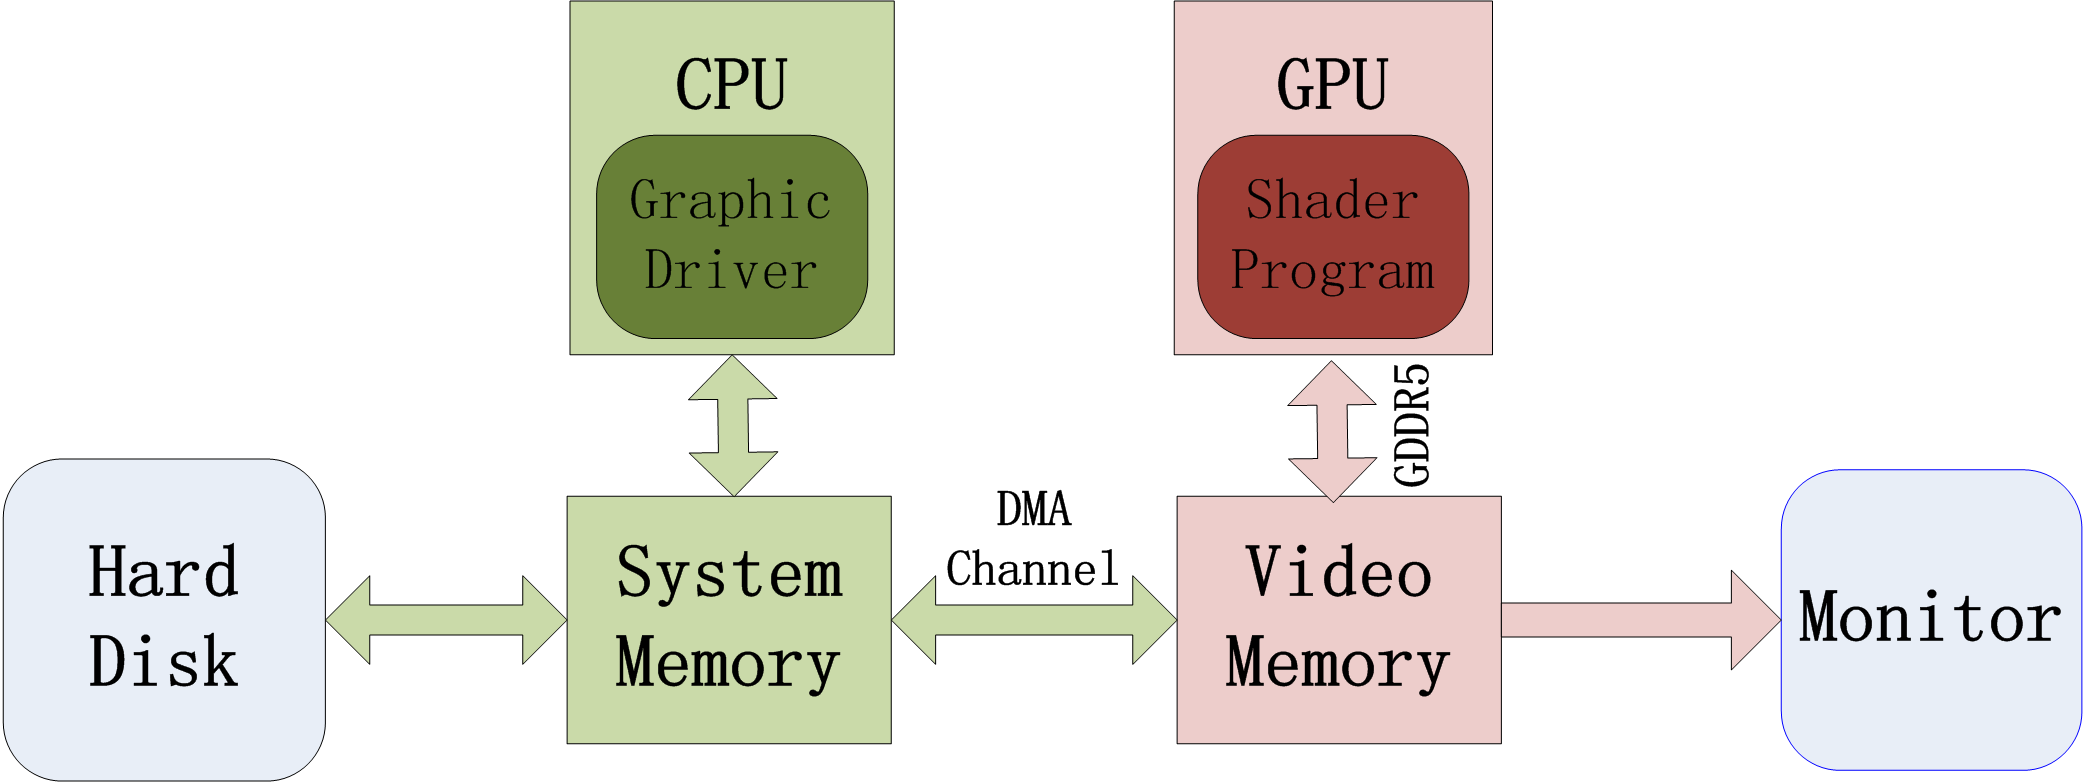
\includegraphics[width=3.4 in]{pics/gpu_render.png}
\caption{GPU game rendering procedure}
\label{fig:gpu_render}
\end{figure}


Modern graphic pipelines are fully programmable. They
execute shader programs which are often compiled
into an intermediate bytecode represented by either the API
library or a front-end part of the driver.
The graphic driver is responsible for keeping track of the API states and translating API calls
into native commands the GPU hardware understands. Furthermore,
the driver requests space for object allocation from either its
own privileged component or the operating system kernel and
decides where and how those objects should reside in the system
or the video memory \cite{gem} \cite{atidriver}. The commands and memory objects are written
into specific locations in the video memory from where they get
picked up by the graphic execution engine. The shader
units in the engine can be programmed to render a 3D scene. Interrupts are used to
notify the driver of events like a finished frame execution.

In the graphic system, the memory bandwidth can often be the limiting factor since modern 3D games require huge amount of memory transactions. For example, a GPU requires very high memory throughput with nearly 180 GB/s memory bandwidth
on a GeForce Fermi architecture \cite{gpulatency} while an \emph{Intel
Nehalem} platform operates on a maximum of 32 GB/s \cite{nehalempage}. As shown in Fig. \ref{fig:gpu_render}, there are two places that can be bandwidth intensive. The first one is the DMA channel between the system memory and video memory limited by the maximum bandwidth of PCIE buses. The second one is the memory buses between the video memory and the GPU core. The limitation here is the bandwidth of GDDR5 data rate.


\subsection {Cloud Gaming}

Cloud gaming aims to provide end users frictionless and direct play-ability of games across various devices \cite{wiki}. The user usually operates the game through a thin client on mobile devices. The controls from the users are transmitted to the cloud server. The graphics cards in the server rack will be responsible for rendering the game instance for each user. After that, the screen frames of the game will be captured and compressed by the video encoding unit and send to the user end through the broadband network. The user client decodes the video stream and playback on the screen. Cloud gaming allows ordinary users to access the demanding high-end games without the need to acquire a powerful game console or computer. However, cloud gaming significantly relies on broadband connection beyond 5Mbps which is not commonly available until recent years \cite{chen14:cloud_gaming_qos}\cite{chen11:cloudgaming}.

GPU resource management in the virtualized cloud gaming
environment is not well studied. Resource sharing in the existing
virtualization solutions is often poor. For example, OnLive allocates one GPU
per game instance \cite{OnLive}. Proprietary motherboards
are also used to host more GPU chips in one server. Due to the complexity of the GPU devices, hypervisors that support GPU paravirtualization
achieve near-native efficiency only recently \cite{nvgrid} \cite{vm}.

 \begin{figure}
\centering
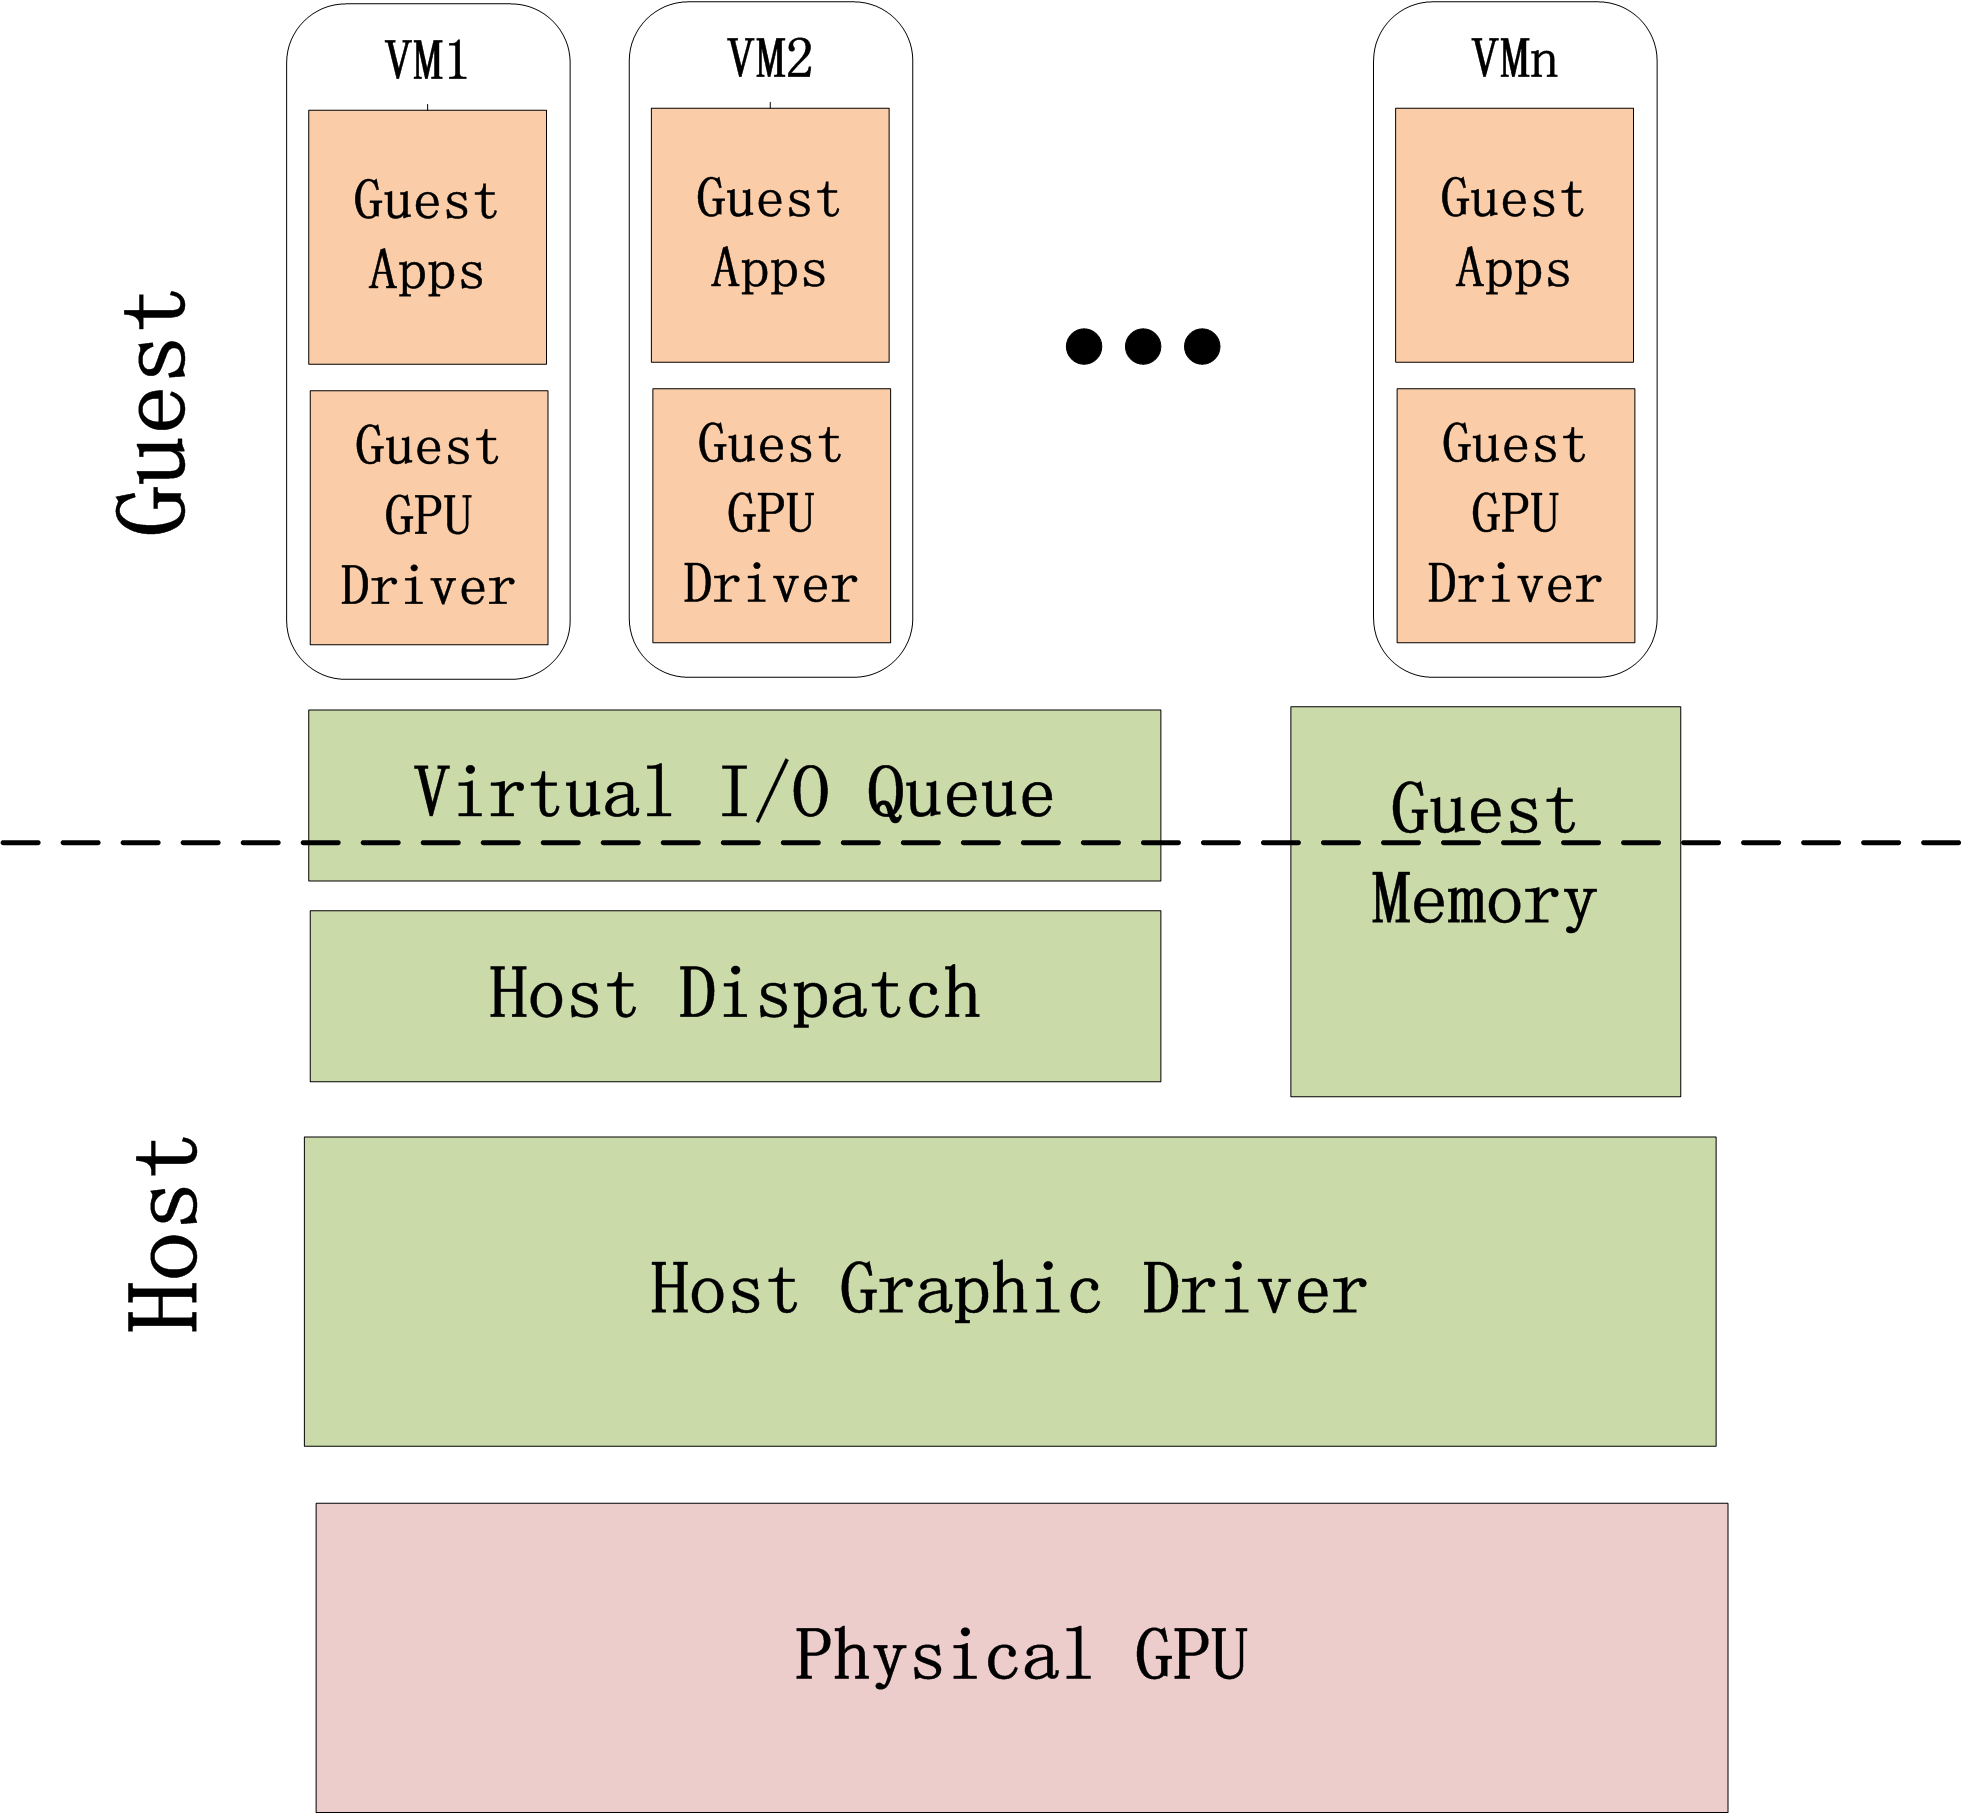
\includegraphics[width=3.4 in]{pics/vm.png}
\caption{Cloud gaming virtualization framework}
\label{fig:vm}
\end{figure}

As shown in Fig. \ref{fig:vm}, in a multi-user cloud gaming server, each guest
application invokes a standard rendering API and the
guest GPU driver prepares the corresponding objects in the guest memory
and issues the GPU command packets. These packets are
pushed into a virtual I/O queue which are subsequently
processed by the dispatch unit in the host. Lastly, this
dispatch layer sends the commands to the host graphic driver in an
asynchronous manner. Objects and contents in the guest memory
are transferred to the physical GPU video memory under the control of the host driver. Multiple-users invoke multiple game instances requiring multiple virtual machines to communicate with the driver.


  \begin{figure}
\centering
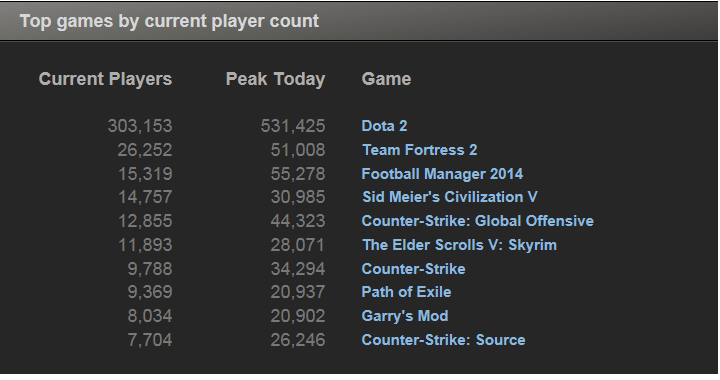
\includegraphics[width=3.5 in]{pics/topgame.png}
\caption{Concurrent players for the top 10 games at a popular gaming site}
\label{fig:topgame}
\end{figure}


The popular task scheduling
mechanisms such as VMWare Player \cite{vm} tend to allocate
GPU resources in a first-come first-serve manner. The host GPU driver once received the request will transfer the corresponding memory objects and run the game instance on the graphic engine. For frame-based scheduling, the GPU will render one game instance for a few frames, perform a context switching and continue to render another game. For time-based scheduling, the GPU will follow the same routine but render a game for a pre-defined time slot. Whenever the GPU performs a context switching for a new game instance, the entire graphic pipeline including all the cache hierarchy is completely flushed \cite{flush1}\cite{flush2}.

\section{Static Analysis}\label{sec:analysis}

 In the cloud gaming environment, it is common that multiple users are playing the same game simultaneously. For example, in many sports and action games, players often team up to play against each other. For popular single-player strategy games, it is also likely that multiple users are playing the same game (multiple copies) at the same time. Fig. \ref{fig:topgame} is a screen capture showing the real-time and peak number of users playing the top 10 games offered by a popular on-line gaming vendor ``SteamPowered'' \cite{steampowered}. The site has 6 millions active users and half of them are playing the top 10 games. About 300K users were playing the most popular game ``Dota2'' at the time we captured the screen. The peak players can be around 500K for this game. This means there are 500K copies of the same game being rendered at the same time in the cloud center. Today's gaming servers leverage graphic cards designed for single game so that the GPU will treat every instance of the same game as independent and render separately. However, the phenomenon in cloud gaming creates a unique opportunity for content sharing between users if multiple copies of the same game are being rendered on the same GPU.

In this section, we focus on static analysis of graphic API calls to measure duplicated data transfers from the system main memory into GPU video memory when multiple users are rendering the same game using the same GPU. We complete our evaluation by doing a static analysis on the traces collected by OpenGL API calls. It enables us to give a quantitative analysis on the potential improvement that one part of our optimizations may achieve. We use ``APITrace'' to do the job \cite{apitrace}. APITrace is a viable tool to intercept calls to graphic driver and store their contents in a reproducible and accessible format. A trace created by APITrace contains all relevant information to reproduce the same rendering that occurred during the original execution of the targeted program as in function names, arguments, data buffers and function return values. The trace is analyzed by identifying and inspecting draw calls that would trigger the data transfer between the system memory and GPU memory that will show us how many redundant transactions can be avoided.

We aim to share the contents among different instances of the same game. There are three major types of contents that can be shared:
\begin{itemize}


\item {The object primitives: these are the primitives (triangles, dots, lines) constructing an object model (car, tree, animal, human, etc.) in a 3D scene. Since multiple copies of the same game are being rendered, it is likely that the same objects will appear.}
\item {The texture map: this is texture (wood, gold, water, etc) used for rendering objects. Texture maps are generally large and take up significant portion of the memory space and bandwidth. For the same reason, it is likely the texture maps can be shared.}
\item {The shader program: this is the program instructing the graphic engine to do the rendering computation. Since it is basically the same game, it is also likely that shader programs can be shared across multiple instances.}

\end{itemize}

 In this paper, we focus on only sharing the texture data because it is memory hungry. The application of our technique to the object primitives and shader programs are trivial. OpenGL provides the programmers with buffer objects that can be declared with usage hints -- \textbf{Static} (texture once loaded never changes); \textbf{Dynamic} (texture changes once in a while); \textbf{Stream} (texture changes frequently) \cite{oglhints}. It is highly possible to share static textures while the chance of sharing dynamic and stream textures is relatively low. Fortunately, the usage hints in OpenGL make life much easier to identify what to share in a game. To show how much of the texture data can be shared with another instance of the game, we sequentially went through two traces collected from two individual players, captured the contents of every data transfer and compared them for redundant occurrences. Note that although the two player were playing the same game simultaneously, the collected traces and the real-time frames displayed on their monitors can be quite different. Fig. \ref{fig:quakeFrames} shows frame \#45 of both user's screens that didn't look alike, but there were still a lot to share in the underlying GPU hardware. This is understandable because both copies of the game use the same texture and materials to render wall, floor, doors and gun, etc. These would the same contents for the same game.

 \begin{figure}[!t]
\centering
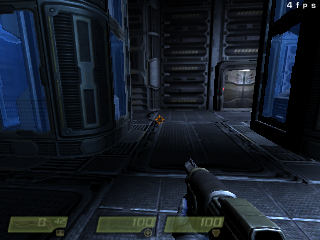
\includegraphics[width=1.6in]{pics/quakeFrame90.png}
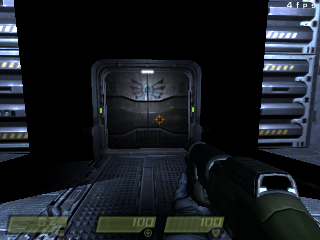
\includegraphics[width=1.6in]{pics/quakeFrame91.png}
\caption{Quake 4 frame \#45 of trace 0 and 1}
\label{fig:quakeFrames}
\end{figure}

	
	\begin{table}[ht]
	  \centering
	  \begin{tabular}{|l|l|l|}
		\hline
		& \multicolumn{2}{c|}{\textbf{Situation}}\\\cline{1-2}\cline{2-3}
		\textbf{Game} & Same scenario& Different scenarios\\
		\hline
		\hline
		TF2&43.95\%(53MB)&40.08\%(51MB)\\
		\hline
		A:TDD&27.64\%(19MB)&17.31\%(8MB)\\
		\hline
		UT2K4&69.66\%(49MB)&53.37\%(35MB)\\
		\hline
        Doom3&49.93\%(55MB)&45.47\%(49MB)\\
		\hline
        Q4A&39.91\%(28MB)&32.39\%(24MB)\\
		\hline
        Prey&51.03\%(36MB)&44.98\%(30MB)\\
		\hline
	  \end{tabular}
	  \caption{OpenGL static analysis for 6 games: ``Team Fortress 2'', ``Amnesia: The Dark Descent'', ``Unreal Tournament 2004'', ``Doom 3'', ``Quake 4 Arena'', ``Prey''}
	  \label{table:analysis}
	\end{table}
%	\begin{table}[h!]
%	  \centering
%	  \begin{tabular}{|l|l|}
%		\hline
%		\textbf{Game scenario} & \textbf{Redundant static data}\\
%		\hline
%		\hline
%		Single run & 9.15 \% (5 MB)\\
%		\hline
%		Same scenario played twice & 43.95\% (53 MB)\\
%		\hline
%		Two different scenarios & 40.08\% (51 MB)\\
%		\hline
%	  \end{tabular}
%	  \caption{\emph{Team Fortress 2} OpenGL trace analysis.}
%	  \label{table:api_tf2}
%	\end{table}
%	\begin{table}[h!]
%	  \centering
%	  \begin{tabular}{|l|l|}
%		\hline
%		\textbf{Game scenario} & \textbf{Redundant static data}\\
%		\hline
%		\hline
%		Single run & 15.26 \% (2.49 MB)\\
%		\hline
%		Same scenario played twice & 57.64\% (18.82 MB)\\
%		\hline
%		Two different scenarios & 17.31\% (8.45 MB)\\
%		\hline
%	  \end{tabular}
%	  \caption{\emph{Amnesia: The Dark Descent} OpenGL trace analysis.}
%	  \label{table:api_amnesia}
%	
We analyze data from six popular games each with two players. For each game we analyze two different situations:

	\begin{itemize}
		\item {\emph{Same scenario}: Two players are playing the same part/stage of a game. This is typically the case that players team up and co-play a game. For example, up to 10 users can join a single basketball match.}
		\item {\emph{Different scenarios}: Two players are playing completely different parts/stages of a game. This is typically the case that people play the same game independently. For example, user A is playing the first stage of ``Doom 3'' while user B is playing the fourth stage.}
	\end{itemize}


	Tab. \ref{table:analysis} shows the percentage and volume of duplicate texture data transfers between the system and video memory in two seconds play time of each game. For most cases with two players, we observer a large number of redundant data transactions ranging from 30\% to 70\%, regardless of \emph{same scenario} or \emph{different scenarios}. The static analysis shows the great potential to eliminate the unnecessary memory and bus operations that can save significant portion of the system bandwidth and memory space. The only exception is in the case of ``Amnesia: The Dark Descent''. This game has extremely fast-changing scenes and large variance across so that the data duplication rate is low.


\section{System and Architecture Changes} \label{sec:contributions}

In order to efficiently utilize the potential benefit of content sharing, we device system and architecture modifications that can be combined to
achieve the optimal results. The first set of changes affects the driver software design that controls how the GPU
hardware handles memory transfers. This solution offers a transparent
usage of the existing software stacks and games at the expense of slightly
increased CPU computation. But it brings the significant advantage of saved memory transactions and space. The second change needs to change GPU cache design. This kind of hardware modifications has to be implemented by the GPU vendor. The overall driver and hardware changes are minimal.

\subsection{System Change: GPU Driver Modifications}

Our scheme relies on being able to identify texture maps that are duplicated. We want to save DMA transfers from the main memory to video
memory and allocate less video memory space for the texture. This means we need the capability to check the data equivalence in the memory.
To take advantage of the existing software stack, we
propose the following driver changes to achieve the best efficiency
while maintaining the system compatibility.

The way we do it is straightforward. The driver captures API calls from the virtualization layer and identifies different types of texture data through the usage hints. Direct3D uses a ``buffer descriptor structure'' to propagate properties of
	a data buffer to the GPU driver. It is used whenever a new memory buffer needs
	to be allocated. This structure contains a usage hint, as already described in
	Section \ref{sec:analysis}. In OpenGL, a memory buffer can be allocated using a call to
	``glBufferData'', which takes a target, buffer size, data and a usage hint
	as the inputs. In both cases, the driver can easily identify the type (texture or not) of memory object to be created and its characteristic (static, dynamic or stream).

As described in Section \ref{sec:analysis}, static textures are easy to share because they are relatively stable. Dynamic and stream textures are hard to share because they vary frequently. So in our design the driver will always transfer the dynamic and stream textures while the static textures will need further processing as shown in Fig. \ref{fig:flow}

 \begin{figure}
\centering
\vspace{-0.5in}
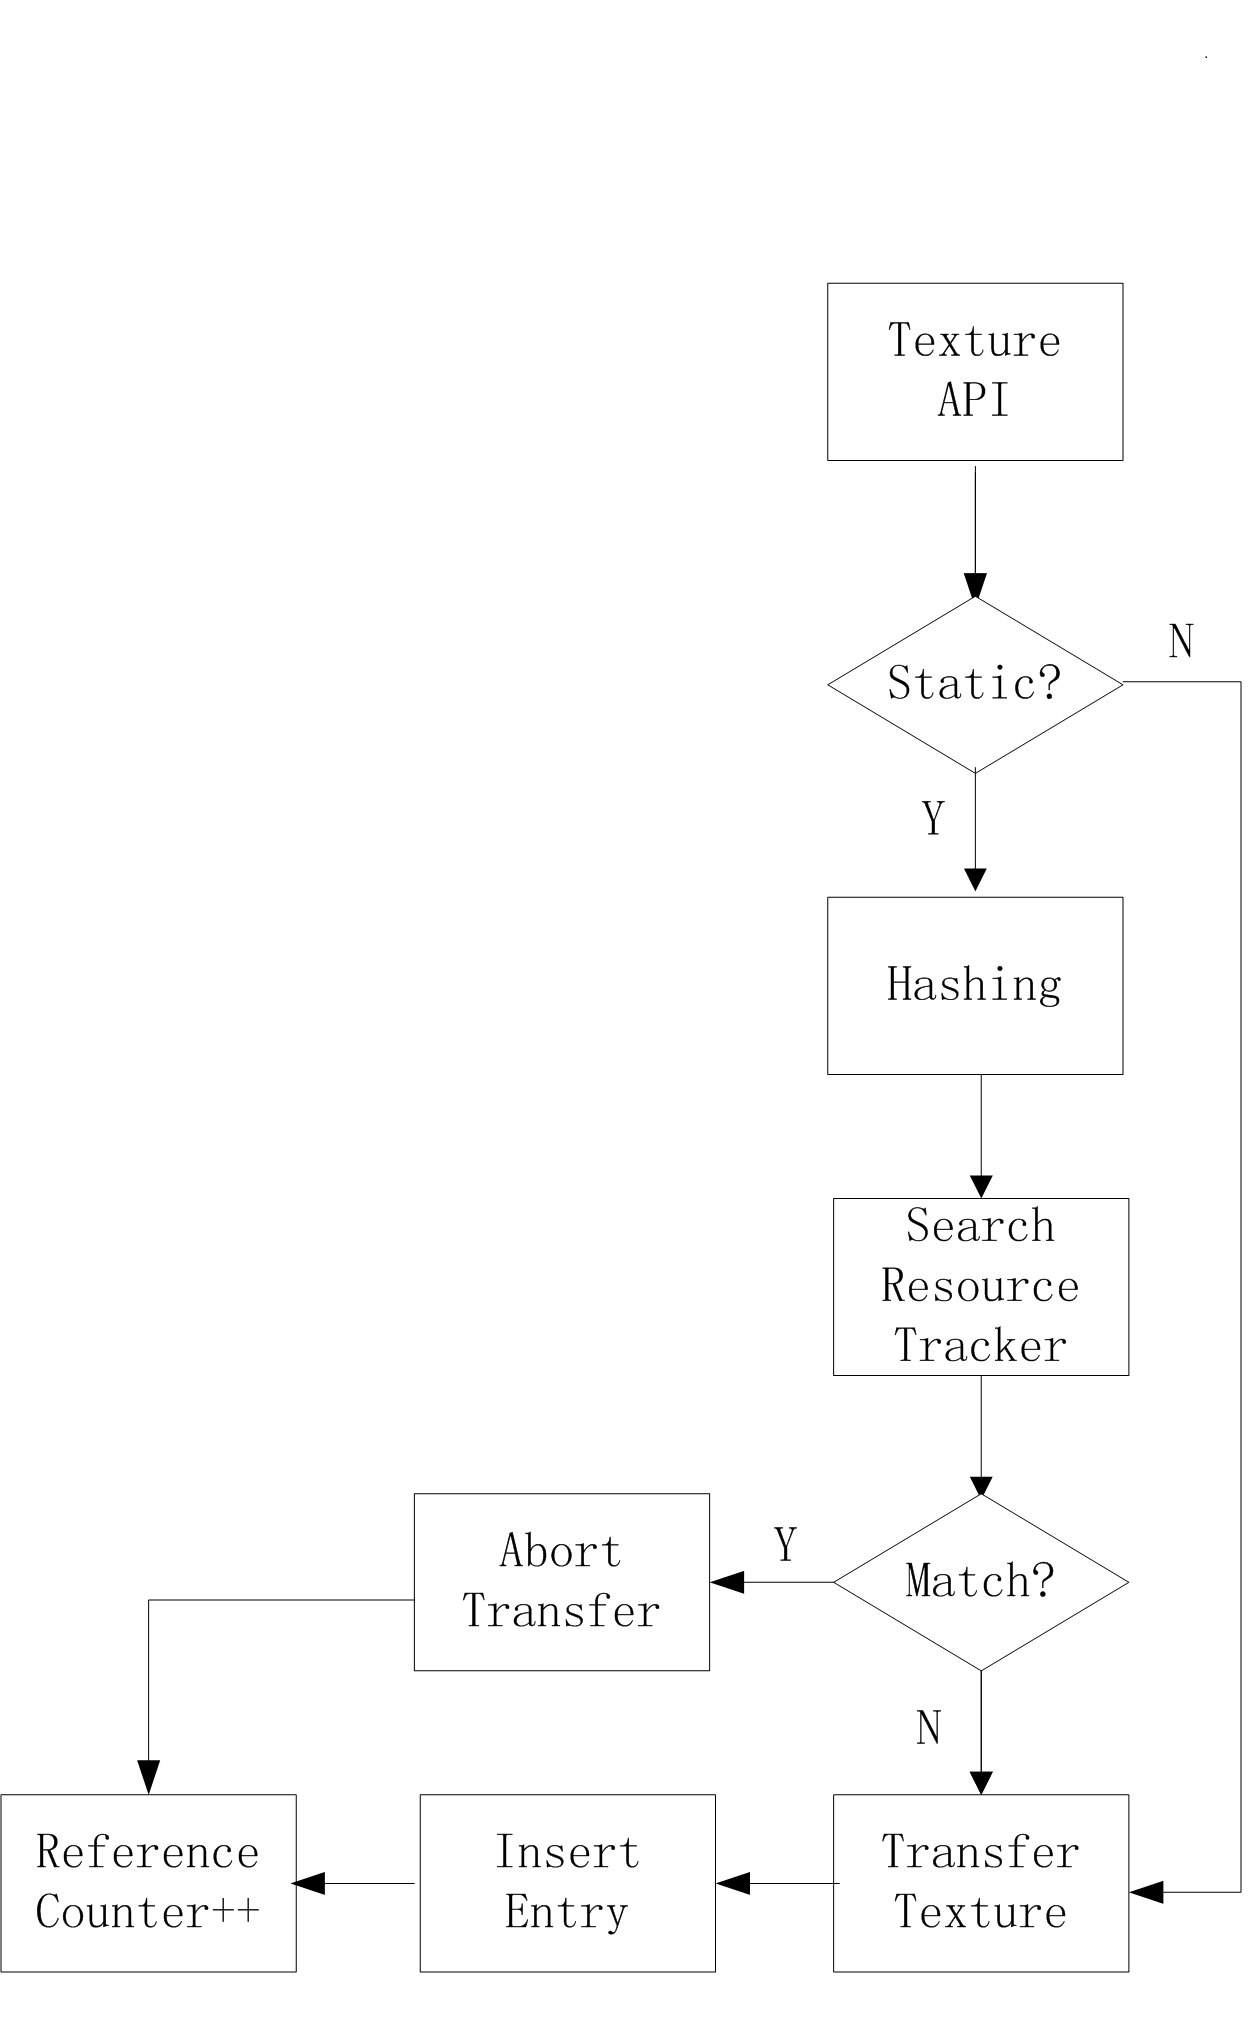
\includegraphics[width=2.6in]{pics/flow.png}
\caption{The program flow implemented in the driver}
\label{fig:flow}
\end{figure}

We modify the driver that is responsible for allocating/deallocating video memory and controls the memory transfers. To be more specific, we
add a resource tracker into the driver that keeps track of all the texture maps having been
allocated in the video memory. The tracker is basically a mapping table stored in the system memory with every entry containing a unique
texture ID as the key and a video memory descriptor and a reference counter as
the corresponding value pair. The memory descriptor is a pointer to the exact location in the video memory where the corresponding texture map is stored. It will be returned when the texture is being requested by the graphic engine in order to locate the texture contents in the video memory. The
reference counter is used to record the number of draw calls which actively use this texture.

In the conventional method, whenever the game API attempts to load a texture, the driver will just allocate the video memory space and transfer the texture data over to the video memory. In our modified driver as shown in Fig. \ref{fig:flow}, it will first check through
the resource tracker to see if it is already present in the video memory by comparing with the texture ID. If there is a match, this means another copy of the game has already loaded the same texture into the video memory and the texture content can be shared. In this case, the driver will abort the texture transfer but instead transfer the video memory descriptor to the GPU. Later if the graphic pipeline wants to render the texture, it can just use the descriptor to find the shared content. This kind of sharing can save significant amount of redundant data transfers and video memory space. The driver also increments the reference counter by one after the process.


It is important to assign a unique ID for every texture so that the driver can easily identify a match in the tracker. The way we choose is to hash the texture and obtain a hash value as the texture ID. We use the ``Murmur Hash'' as the hash function \cite{michail2009top}, since it is a very popular and efficient
way of hashing non-cryptographic data. A match of the texture ID means the same texture has already been loaded into the video memory. The hashing function is part of the driver and takes CPU cycles. It is executed every time a static texture is requested by the game API. The hashing can potentially degrade the system performance, but we will show in Section 6 that the saved memory transfer time can well offset the hashing overhead and result in an overall system performance gain.


Whenever there is a miss in the tracker which means there is no existing matching texture in the video memory, the texture will be transferred and an entry will be inserted into the tracker. In case the amount of the video memory space is below a threshold, we need to free some memory first. The driver chooses the victim texture based on the values in the reference counters. The driver will always invalidate the texture with the smallest reference counter value which means this texture is least frequently used and discarding it may not have big impact.

\section{Experiment Setup}\label{sec:details}

In this section we will discuss our experiment setup. We will start by
explaining our undertaken changes to the Gdev driver on a real cloud gaming server and the ATTILA GPU simulator.

\subsection{Real System Setup}
We build a real cloud gaming system with the configurations shown in Tab. \ref{table:simulationPC}. We assume two users and setup two virtual machines with each owning two cores and 2GB main memory. Ubuntu 12.04 linux OS is used as the operating system for both the host and
guests. We use VMWare \cite{vm} as the paravirtualization software.


 \begin{table}[h!]
	\centering
	\begin{tabular}{|l|l|}
		\hline
		\textbf{Parameter} & \textbf{Value} \\
		\hline
		\hline
		CPU & AMD Athlon X4 Quad-core 631 2.6 GHz \\
		\hline
		Memory & 16G DDR3-1333 Dual-Channel \\
		\hline
		Mainboard & Biostar A55 chipset \\
		\hline
		Graphics Card & Inno3D Geforce GT440 1GB \\
		\hline
		CUDA core & 96 \\
		\hline
		GPU frequency & 810 MHz \\
		\hline
		GPU memory & 1GB GDDR5 @ 3200MHz 128bit \\
		\hline
	\end{tabular}
	\caption{Gaming System Parameters}
	\label{table:simulationPC}
\end{table}

Most of the system hacks lay in the host graphic driver layer as shown in Fig. \ref{fig:vm}. Because the driver design is the top secret for graphic card vendors like NVIDIA and AMD, we have to leverage the open source GPU driver ``Gdev'' \cite{gdevpaper} to evaluate the impact of our technique on a real system. Gdev is a GPU runtime and resource management engine that enables flexible GPU control and tuning. Gdev has an option to define shared memory area in the GPU which greatly facilitates our goal to allow game instances to share data and avoid unnecessary memory transfers. The interface is based on the standard SysV IPC \cite{gdevpaper}.

We use software to record the real-time frames per second of each game. This is the direct reflection of the gaming performance. We also use software to record the memory transactions and memory usage. If needed, we use a multi-meter to measure the current flowing through the GPU card and calculate the power consumption. Fig. \ref{fig:test} is a snippet of our system.

 \begin{figure}
\centering
\includegraphics[width=2.8 in]{pics/test.jpg}
\caption{The cloud gaming system used for the experiments}
\label{fig:test}
\end{figure}

\subsection{GPU Simulation Setup}

Since we cannot add hardware features into the graphic card, we have to leverage a GPU simulator to exploit the architecture changes we proposed such as the enhanced cache designs. We use ``ATTILA'' \cite{attilapaper}, a detailed open source end-to-end graphic pipeline simulator which can report hardware status such as pipeline and cache behavior. ATTILA was originally developed to simulate a single trace. In order to simulate
content sharing among multiple games, we extend the functionality to
allow ATTILA to run multiple traces with a context switch at the end of every rendering period. The crucial ATTILA simulation parameters are listed in Tab. \ref{table:simulationParameters}.


\begin{table}[h!]
	\centering
	\begin{tabular}{|l|l|}
		\hline
		\textbf{Parameter} & \textbf{Value} \\
		\hline
		\hline
		GPU Clock & 500 MHz \\
		\hline
		Shader Clock & 500 MHz \\
		\hline
		Memory Clock & 500 MHz \\
		\hline
		Memory Size & 256 MB \\
		\hline
		Vertex Shaders & 8 \\
		\hline
		Fragment Shaders & 4 \\
		\hline
		Streamer Unit Cache Lines & 32 \\
		\hline
		Streamer Unit Cache Line Size & 256 Bytes \\
		\hline
		Texture Unit L0 Cache Lines & 8 \\
		\hline
		Texture Unit L0 Cache Line Size & 64 Bytes \\
		\hline
		Texture Unit L1 Cache Lines & 32 \\
		\hline
		Texture Unit L1 Cache Line Size & 64 Bytes \\
		\hline
		Texture Size & 4*4 pixels, 64 Bytes \\
		\hline
	\end{tabular}
	\caption{ATTILA Simulation Parameters}
	\label{table:simulationParameters}
\end{table}


\subsection{Description of Games}

We use 6 popular games in our experiment. The games cover a wide range of arena scenes, modeling styles and texture types. They are described as follows:
\begin{itemize}
	\item \emph{Team Fortress 2}: a team-based multi-player game developed by Valve Corporation. Team Fortress 2 is focused around two opposing teams competing for a combat-based principal objective. Players can choose to play as one of the nine classes in these teams, each with his own unique skills.
	\item \emph{Amnesia: The Dark Descent}: a survival horror game by Frictional Games. The game features a protagonist exploring a dark and foreboding castle while avoiding monsters and other obstructions as well as solving puzzles.
    \item \emph{Unreal Tournament 2004}: a futuristic first-person shooting game developed by Epic Games and Digital Extremes. It is part of the Unreal series, particularly the subseries started by the original Unreal Tournament.
    \item \emph{Doom 3}: a science fiction game developed by id Software. The game was a huge success with more than 3.5 million copies sold. Critics praised the game's outstanding graphics and presentation.
    \item \emph{Quake 4}: the fourth title in the series of Quake. The game was developed by Raven Software. id Software supervised the development of the game as well as providing the Doom 3 engine.
    \item \emph{Prey}: a first-person shooting game developed by Human Head Studios. Prey uses a heavily modified version of id Tech 4 to use portals and variable gravity to create the environments the player explores.
\end{itemize}

\subsection{Experiment Method}

NVIDIA Grid technology \cite{nvgrid} currently can support two games at a time per GPU. We mimic this by allowing two instances of the same game to run under the \emph{non-sharing} and \emph{sharing} conditions. The \emph{non-sharing} case is the traditional solution that the two game instance will be rendered independently. The \emph{sharing} case utilizes the technology described in this paper and implements the augmented driver for content sharing. We also run the games under \emph{same scenario} and \emph{different scenarios} conditions as described in Section \ref{sec:analysis}.

 \begin{figure*}
\centering
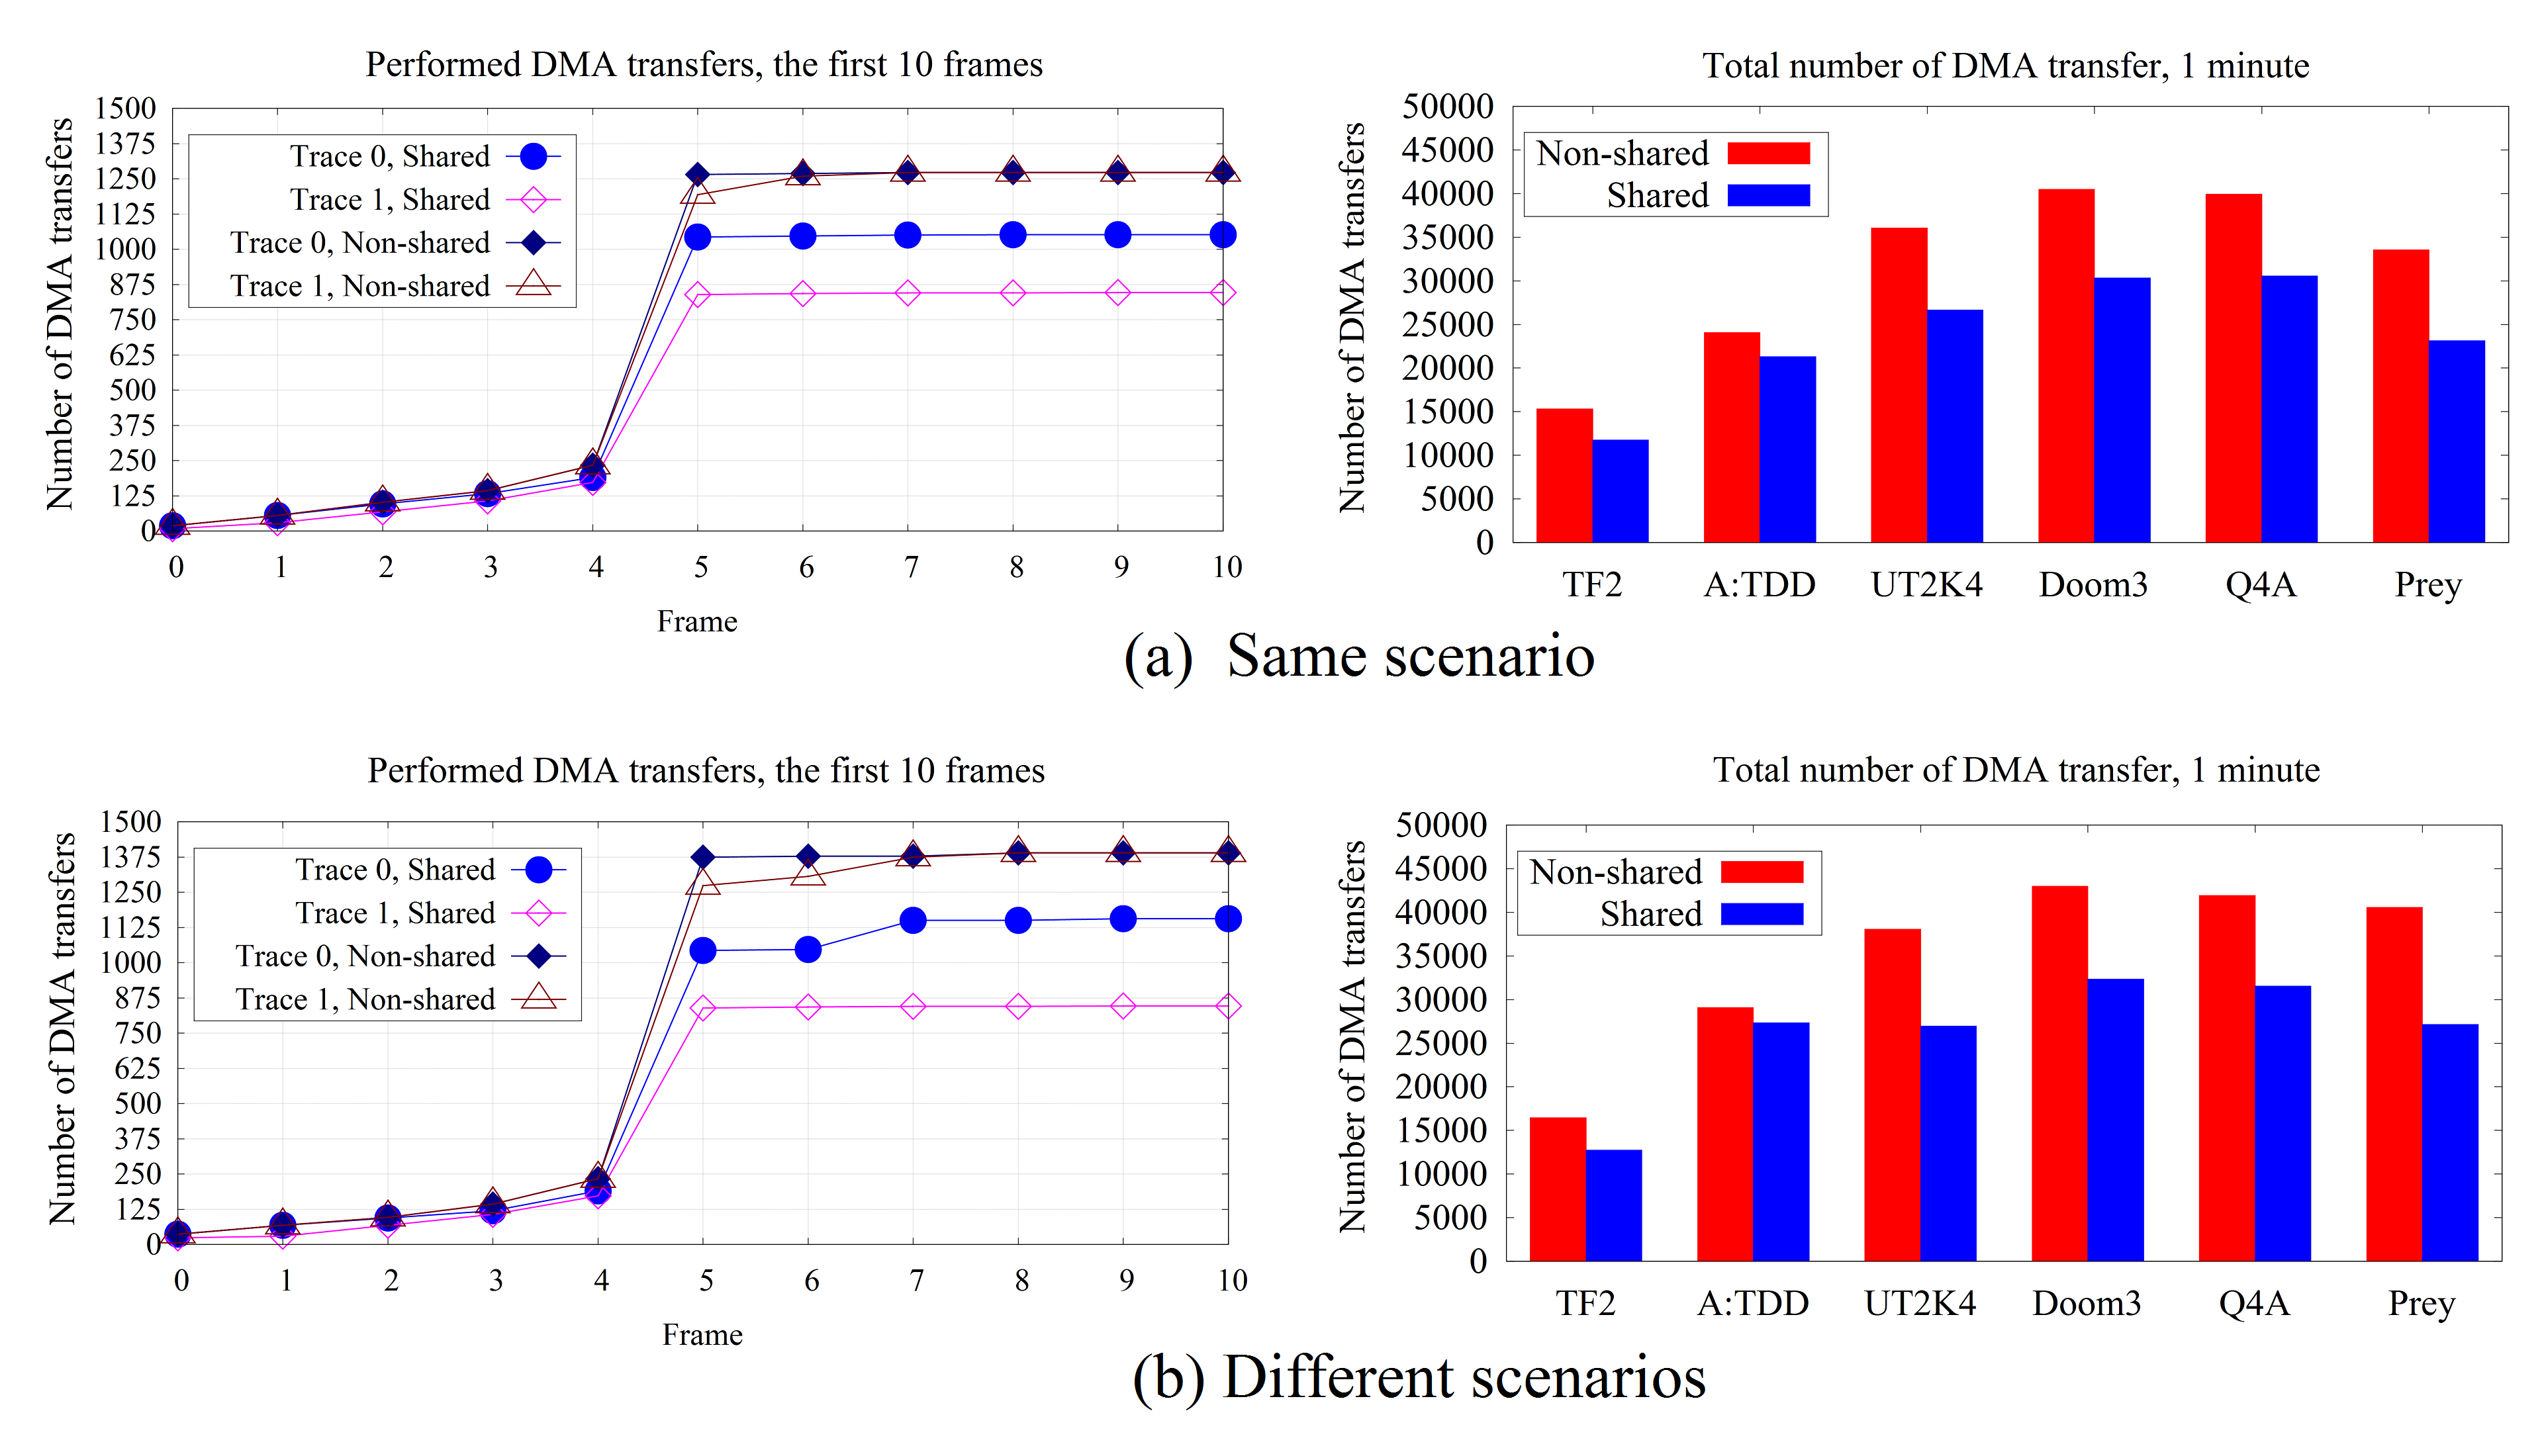
\includegraphics[width=7in]{pics/12.png}
\caption{DMA transfers under different cases}
\label{fig:result1}
\end{figure*}

  \begin{figure*}
\centering
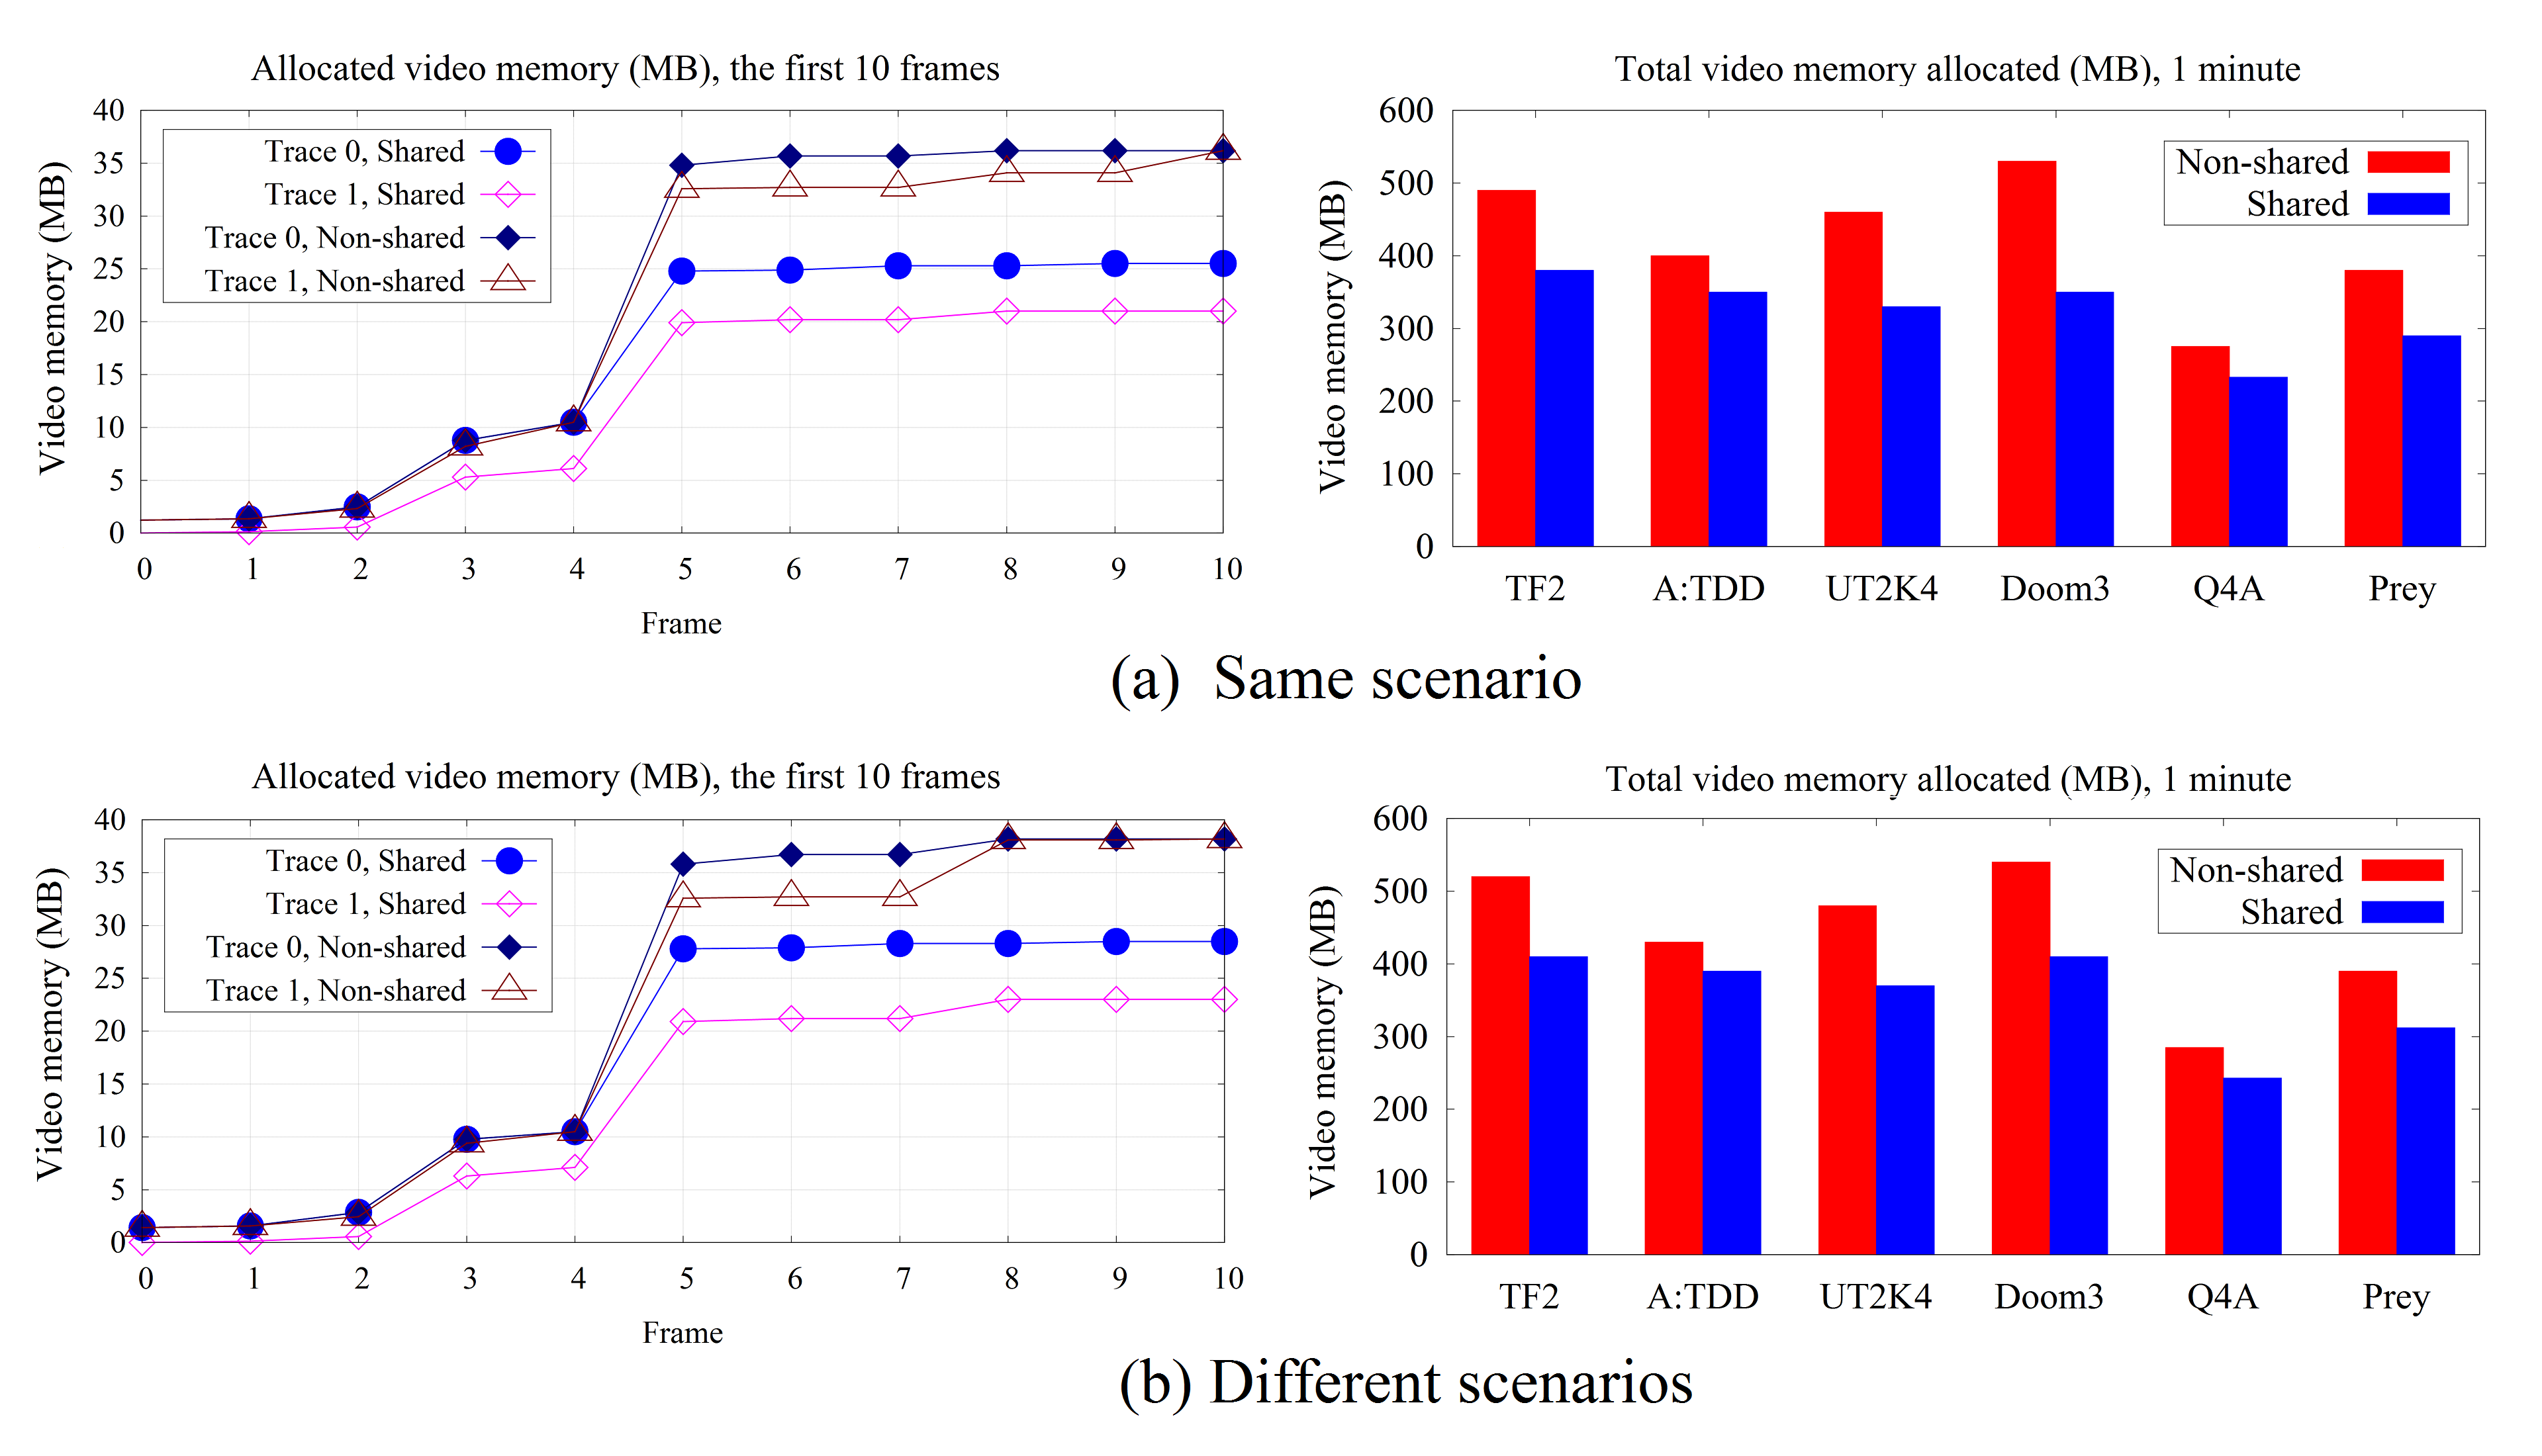
\includegraphics[width=7in]{pics/34.png}
\caption{Allocated video memory under different cases}
\label{fig:result2}
\end{figure*}


\section{Experiment Results}\label{sec:simulation}

In this section we will discuss the impact of content sharing in a GPU-based cloud gaming server.
All the results collected in this section are from the run-time statistics of our cloud gaming system described in Section 5.1 except for the results of caches which are collected from ATTILA simulator.


The left plot in Fig. \ref{fig:result1}(a) shows the aggregated DMA bus transfers
for the first 10 frames of the game ``Quake 4'' under the \emph{same scenario}. We show the two traces from two players under the \emph{sharing} and \emph{non-sharing} conditions. The first 5 frames are the screen loading period so that we see increasing number of static textures. The 6th frame is the first one rendering the actual arena. After that, the screen is stabilized and there are relatively less static textures transfers.
Actually in many games, the majority of static textures is loaded into the video memory in the first couple of frames for rendering the arena. After this initial
burst, not much static texture will be issued from the driver for some time. Obviously in case of
  an arena or level change, a new burst of static textures will occur and in turn call for a new wave of DMA transfers.


 \begin{figure*}
\centering
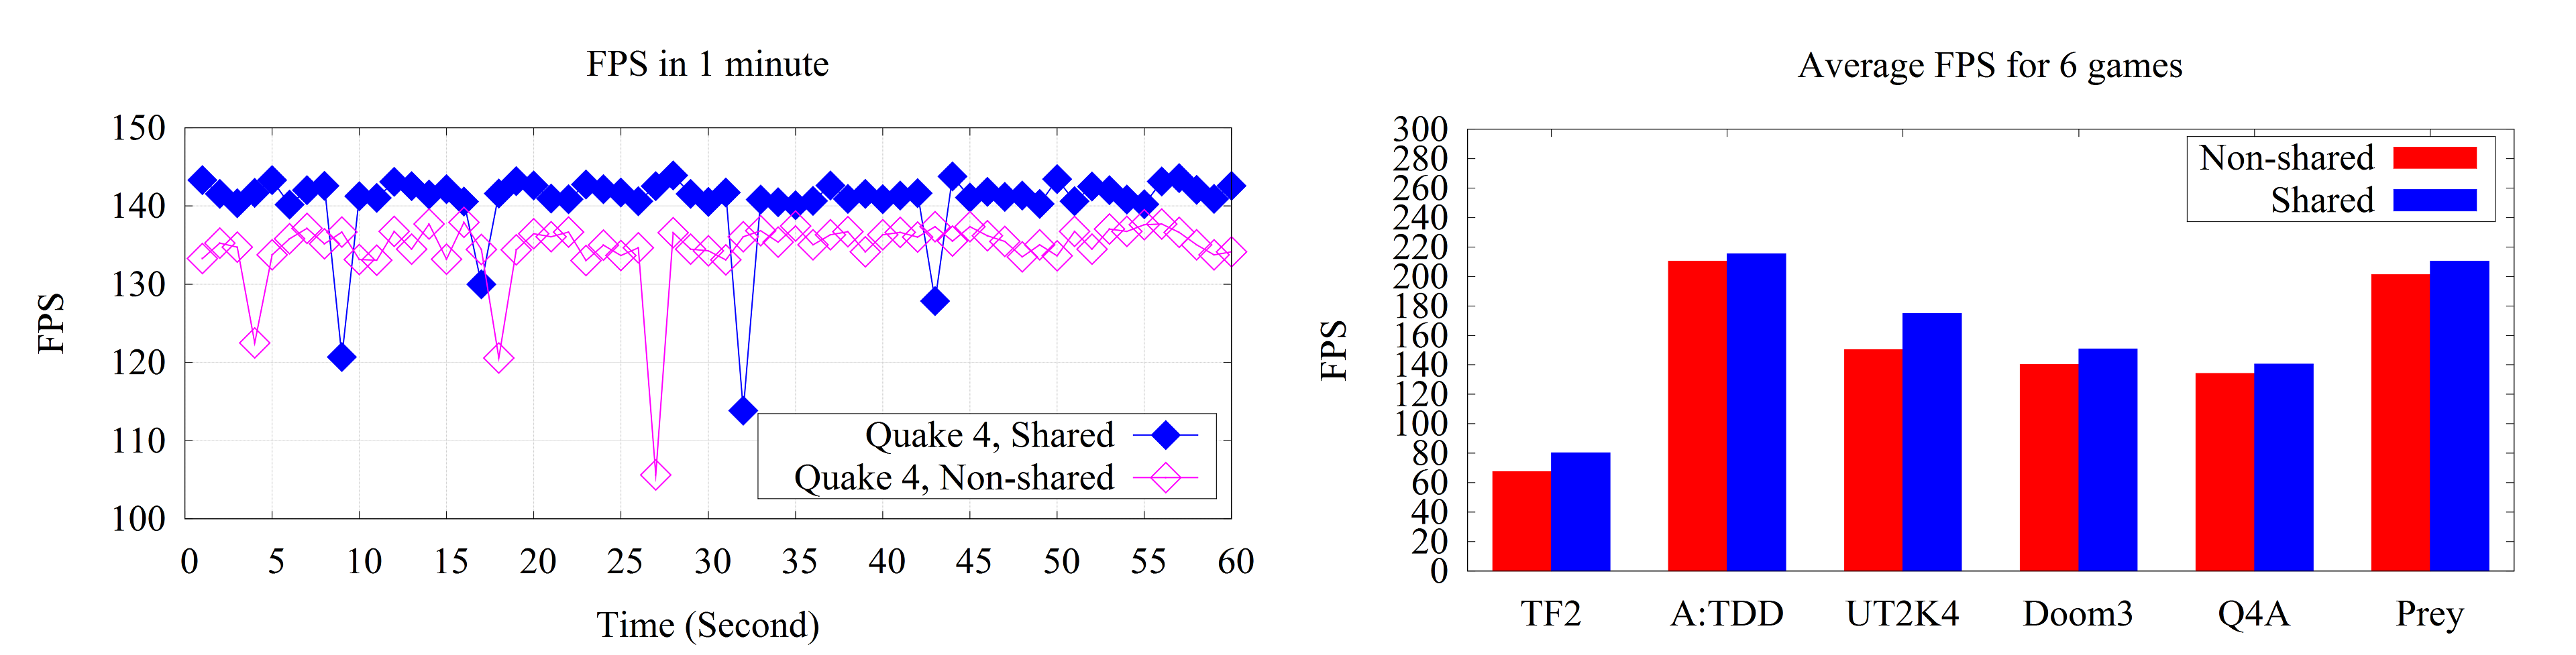
\includegraphics[width=7.4in]{pics/7.png}
\caption{Frames per second under different cases}
\label{fig:result3}
\end{figure*}

 \begin{figure*}
\centering
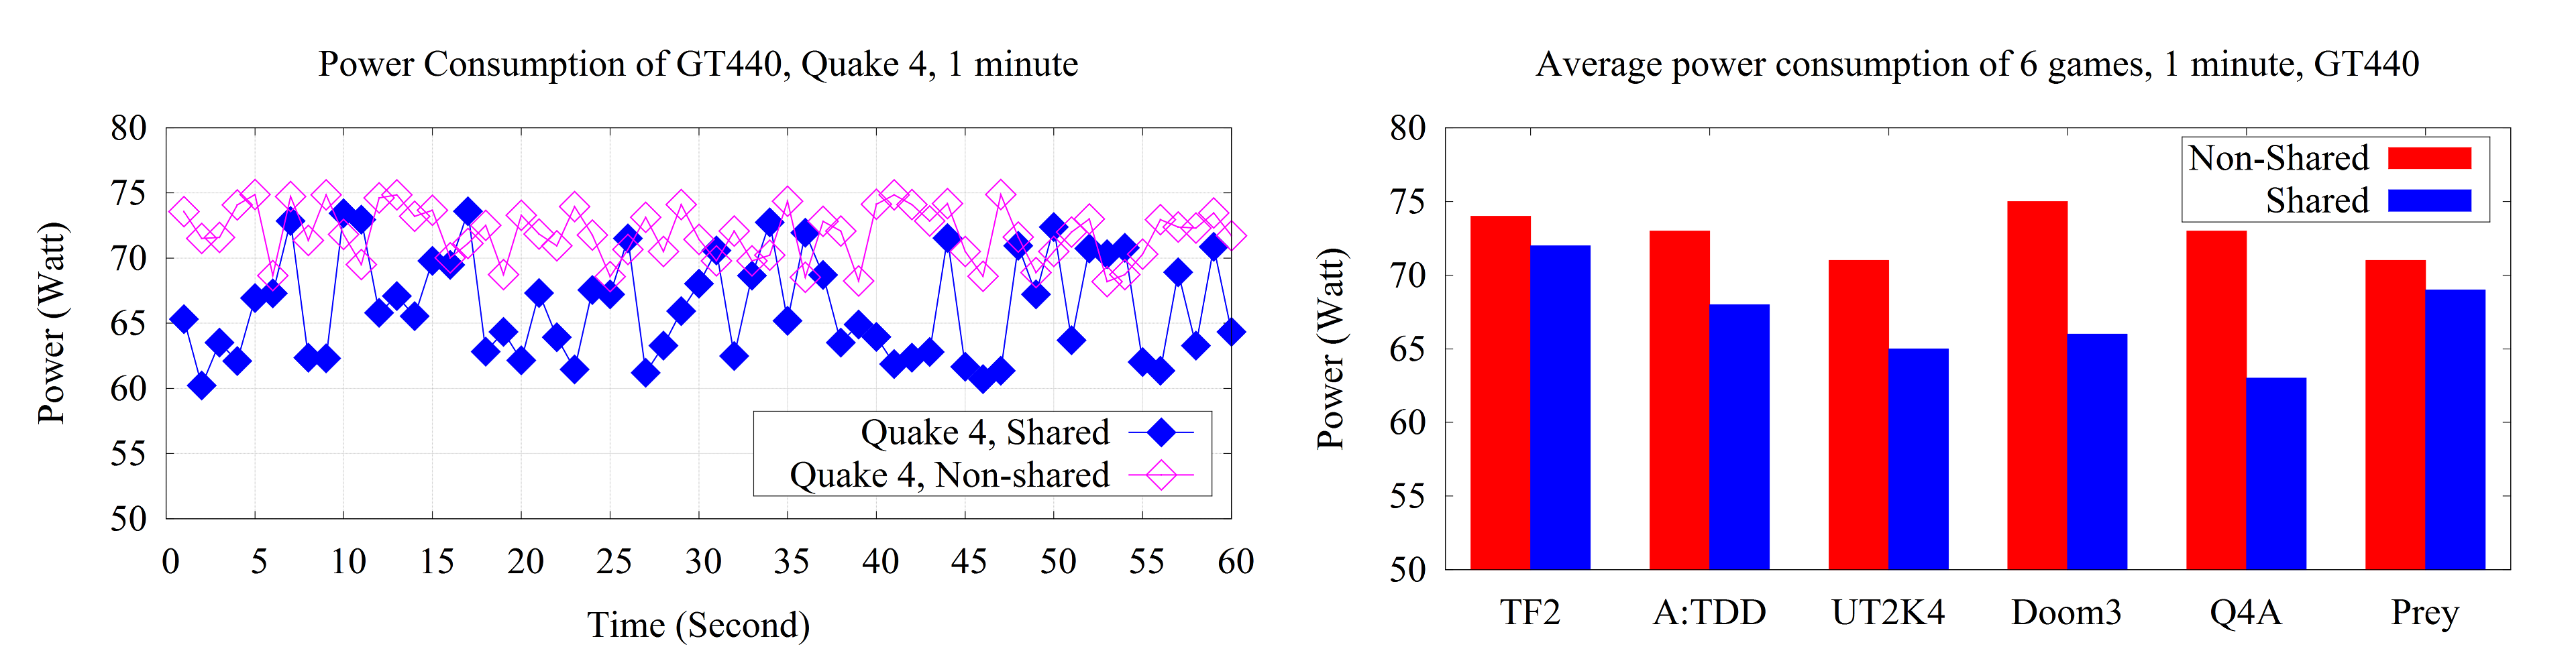
\includegraphics[width=7.4in]{pics/8.png}
\caption{GPU power consumption under different cases}
\label{fig:result4}
\end{figure*}

As shown in the left plot of Fig. \ref{fig:result1}(a), we see that the driver transfers about 20 textures (1.4MB) in the first frame with a big burst in frame 5, where 1030 textures (23MB) are transferred,
In the \emph{non-shared} case, each trace performs
this workload. But for the \emph{shared} case, we are able to reduce the DMA transfers of
the trace 1 by a considerable amount. Trace 0 saves relatively less DMA transfers because it is the first running trace assigned by the driver.
Trace 1 performs only 660 texture transfers in frame 5 compared with the 1030 transfers under the \emph{non-sharing} case. This
means we saved about 45\% of the bus transactions for trace 1. In the right plot of Fig. \ref{fig:result1}(a), we show the long-term behaviour of all the six games. This shows the aggregated DMA transfers for one minute of game play. The game ``A:TDD'' doesn't perform well because the reuse rate of the static textures due to the fast change scenes in this game as discussed in Section \ref{sec:analysis}.


Fig. \ref{fig:result1}(b) shows the same sets of results under \emph{different scenarios}. In this case, sharing content is combined with different gaming environment. This test is designed to reveal the true potential of content sharing in the real cloud gaming platform where multiple users are playing the same game but at different scenarios. It is obvious that in the real gaming environment, the gaming arena will keep changing due to the movement of different players. So it is imperative that we analyze the effect of content sharing under this condition. This figure again proves that the high sharing potential of textures is possible even at \emph{different scenarios} of the same game. These results are not surprising as have been seen in Section \ref{sec:analysis}. Even with different arenas, there are still a lot to sharing because the game typically uses the same textures for rendering objects such as walls, floors, water and sky. We find that on average 31.84\% of DMA transfers can be eliminated.


Fig. \ref{fig:result2} shows the allocated video memory space. The left plots are the video memory condition for the first 10 frames. We observe quite similar trend as in Fig. \ref{fig:result1}. Differently, we see relatively staggering lines for the first 5 frames. This is because the texture sizes vary quite a lot and individual frames may incur large variance in the total amount of memory needed for holding the textures. On average for the six games in our experiment, 26.89\% of video memory space can be saved as shown in the right plot of Fig. \ref{fig:result2}. The capacity of the video memory is a precious resource especially under cloud gaming where multiple games divide the entire memory space.



In Fig. \ref{fig:result3}, we analyze the results from the rendering performance point of view. GPU Cycles are one of the most important factors that affect the user experience of a cloud gaming platform. Other factors include network connections, etc. We measure the real-time Frames Per Second (FPS) which is a direct reflection of the game rendering performance. An FPS rate over 30 means no flicking to the human eye but high quality games require an FPS over 60. The left plot in the figure shows the FPS for one minute play time in ``Quake 4''. We observe a constant trend that the \emph {shared} case has a higher FPS than the \emph{non-shared} case. Sharing content incurs overhead in CPU side because the CPU spends more cycles in the driver to do the hashing. But the much saved DMA transfers greatly reduce the memory transaction time so that we observe an overall net gain in the gaming performance. This is essentially important in the future cloud gaming servers when many graphics-intensive instances co-exist so that the system cannot guarantee a constant rate above 30 FPS. Using content sharing will potentially reduce the chance of "lagging or flicking" in the game play. The valleys in the plot is caused by intensive engagement between two players, such as the two players encounter for a fight. This usually imposes rendering pressure on the GPU. For the \emph{non-shared} case, each game instance fetches its own textures and costs memory cycles. For the \emph {shared} case, memory cycles can be saved because of the sharing during the engagement of the players. This again proves the efficiency of our scheme. Overall, the scheme improves the average FPS of the six games by 8.99\% as shown in the right plot of Fig. \ref{fig:result3}.


  Fig. \ref{fig:result4} shows the measured power results. The left plot shows the real-time power measurement for one minute in ``Quake 4''. Sharing content means, to some extent, the power savings since we have eliminated the redundancy. We observer a constant lower power consumption in the \emph {shared} case. The biggest impactor here is the much reduced DMA transfers which can be power hungry. Compared with the \emph {non-shared} case, we see large peaks and valleys in the power consumption of the \emph {shared} case. This is understandable in that the valley usually means the texture intensive period of the game where the \emph {shared} scheme can reduce power consumption by a lot. The peaks typically involves no texture operations so that the power consumption is comparable to the \emph {non-shared} case. We find in an average 8.51\% drop in power consumption of all the six games as is seen in the right plot of Fig. \ref{fig:result4} which proves the better energy efficiency of our scheme.

\section{Related Work}\label{sec:related}

In this section, we survey the existing gaming systems and proposals for better user experiences.
As far as we know, this is the first paper describing the content sharing for common game instances in a GPU-based gaming server. But there are many related works focusing on cloud gaming architecture and measurement of QoS of the cloud gaming systems. We will also introduce related works of GPU resource sharing and virtualization.

\noindent \textbf{A. Cloud gaming architecture}

Cloud gaming systems are generally classified into three categories: (i) 3D graphics streaming \cite{related12} \cite{related19}; (ii)video streaming \cite{related42} \cite{related18}; (iii) video streaming with post-rendering operations \cite{related33} \cite{related16}.

3D graphics streaming approach aims to intercept and compress the graphics commands and stream them to the users. The user clients receive these OpenGL/Direct3D commands and then render the game scenes using its own graphics card. This approach imposes less workload on the cloud gaming server at the cost of more workload on the clients, making cloud gaming on resource-constrained devices almost impossible.

Video Streaming approach \cite{related42} \cite{related18} uses cloud servers to render the 3D graphics commands into 2D videos, compresses the video and then streams them to the target clients. The clients decode and display the corresponding video streams. This approach relieves the clients from rendering-intensive work and can be ported to different platforms.

Video streaming with post-rendering operations \cite{related33} \cite{related16} is a combination of the two methods mentioned above. Most of the rendering are performed in the cloud servers with some post-rendering such as motions, lighting and textures \cite{related6} done on the thin clients.

\noindent \textbf{B. Measuring the QoS of cloud gaming system}

The Quality of Service of cloud gaming system has long been the heated topic in this area. \cite{related20} \cite{related26} give us a slow-motion analysis of an application on the server and the corresponding thin client system. However, slow-motion analysis is flawed for cloud gaming because cloud gaming services are running in real time and a slow-motion analysis can not cover all the behaviors of this service. The performance of thin client based platform has been well investigated including network traces between X-Window server and the clients under different network conditions \cite{related30}. Performance of process, memory and network bandwidth of Windows NT Terminal Service \cite{related43}, as well as the performance of applications running on VNC (Virtual Network Computing) with diversified round-trip times (RTT) \cite{related37} have been well studied. Recently the performance of thin client gaming has been the popular subject of cloud gaming research. \cite{related4} proposed a methodology to study the performance of games on the general-purpose thin clients including LogMeIn \cite{related24}, TeamViewer \cite{related36} and UltraVNC \cite{related38}. \cite{related5} proposed a methodology to quantify the response delay. \cite{related22} evaluated the fairness among different games under cloud gaming settings. \cite{related7} evaluated whether a wide-scale cloud gaming platform is feasible on the current network conditions and proposed a solution to lower user-end delays.


\noindent \textbf{C. GPU resource sharing and virtualization}

There have been some existing ideas on how to use the immense potential of GPUs for better efficiency.
For instance in \cite{gdevpaper}, resource-sharing protocols for the
X-Window System are described to overcome a priority inversion problem for
concurrent access of the same resource.

Further an API named ``Gdev'' \cite{gdevpaper} enables the programmer to
share resources amongst contexts in a Fermi architecture GPU and deal with
enhanced resource management. The main purpose is for computing applications running on GPGPU, whereas our goal
lies in sharing content amongst common games and to show the potential of a
possible gain. The resource management is very helpful since it enables programmers to allocate memory space exceeding the physical size of
the device memory.

Other ideas focus on GPU virtualization where multiple instances try to co-execution in the GPU. Unlike the technique described in this paper where different contexts are time-multiplexing the GPU under the driver's control, the true hardware virtualization tries to achieve space-multiplexing the GPU. In \cite{gpucloudsharing},
the open source framework ``gVirtuS'' \cite{Giunta} is extended to map many
kernels on a GPU concurrently and to calculate an affinity.


\section{Conclusion}\label{sec:conclusion}

In this work we are able to identify the content resources with high sharing
potential in the emerging GPU-based cloud gaming servers where multiple-users can be playing the same game on the same GPU. We also calculate a static estimate on the advantages of sharing the content from different game instances. We enhance system driver design and develop CCP cache replacement policy for the texture cache architecture to further exploit the potential of content sharing GPU in the cloud-gaming environment.
In our research it becomes clear that sharing textures and other memory objects brings
the major advantages in the reduced memory transactions, memory space, power consumption and improved cache hit rate. We also find that the gaming performance has been improved because of the average reduced latency for memory access. Our experiment on the real cloud gaming system and the GPU simulator proves that the proposed techniques can bring significant advantage when comparing with traditional solutions.

In our future work, instead of just sharing the static texture, we will be looking into more efficient ways to share dynamic and stream textures, probably collaborating with the task scheduler. It is also trivial to share object primitives and shader programs following the same scheme. Another interesting question in the future research would be how to share computation. Since multiple players are essentially playing the same game, it is possible to even share some computation besides the memory contents. Sharing computation can greatly reduce the total GPU power consumption and at the same time boost the graphic rendering speed.


\bstctlcite{bstctl:etal, bstctl:nodash, bstctl:simpurl}
\bibliographystyle{IEEEtranS}
\bibliography{references}

\end{document}


